
\newcommand{\etas}{\ensuremath{\eta_{\mathrm{s}}}}


\chapter{Introduction}

The rise of cryptocurrencies have openend up unending possibilities of how minimal or no trust based systems could be established owing to decentralization.
The concept of blockchain was introduced with the founding of Bitcoin by Satoshi Nakamoto \cite{Nakamoto2009}.
Satoshi Nakamoto proposed and implemented idea of a consensus based, trustless, truly peer-to-peer system for financial transactions.  
Notwithstanding an intrumental step towards establishing a decentralized and a trustless system, Bitcoin has several practical limitations with regards to privacy, security and scalability \cite{Conti2018}.   
This led to the development of more privacy and anonymity focussed cryptocurrencies like Monero \cite{Saberhagen2013} and Zcash \cite{Sasson2014}.
Grin \cite{GrinWebsite} and Beam \cite{BeamWebsite} are two relatively new projects which are backed by the MimbleWimble protocol \cite{Poelstra2016} and claim to promise scalability, anonymity and fungibility all at once.
The rise in privacy-centric cryptocurrencies further led to growth in popularity of cryptocurrencies not only among investors but also common people.


\section{What is a Blockchain?}
\label{scn:blockchain}

The concept of a Blockchain originates from the idea of having a decentralized, publicly visible and trust-free ledger.
The term \textit{blockchain} was first coined by Satoshi Nakamoto, the creator of Bitcoin \cite{Nakamoto2009}.
In literal terms, a blockchain implies that blocks containing financial transactions would be added to a publicly verifiable ledger in a timely manner, forming a \textit{chain} of \textit{blocks}.
We expand on the need and the basic idea of a decentralized ledger in the following subsection.

\subsection{Decentralized Ledger}

A ledger is a principal book of records which keeps a track of all transactions measured in terms of a monetary unit. Bitcoin is a decentralized, public ledger, decentralized because there is no trusted third party controlling the ledger and public because anyone with bitcoin can participate in the network, receive and send bitcoins, and even hold a copy of this ledger (essentially, the history of all transactions) if they want to. In that sense, the ledger is ``non-trusted'' and transparent to public. As opposed to such a decentralized ledger setup, traditional banks use centralized ledger system where each bank has it's own ledger visible only to the concerned user.\\ 

\begin{figure}[h!]
    \centering
    \begin{subfigure}[b]{0.5\textwidth}
        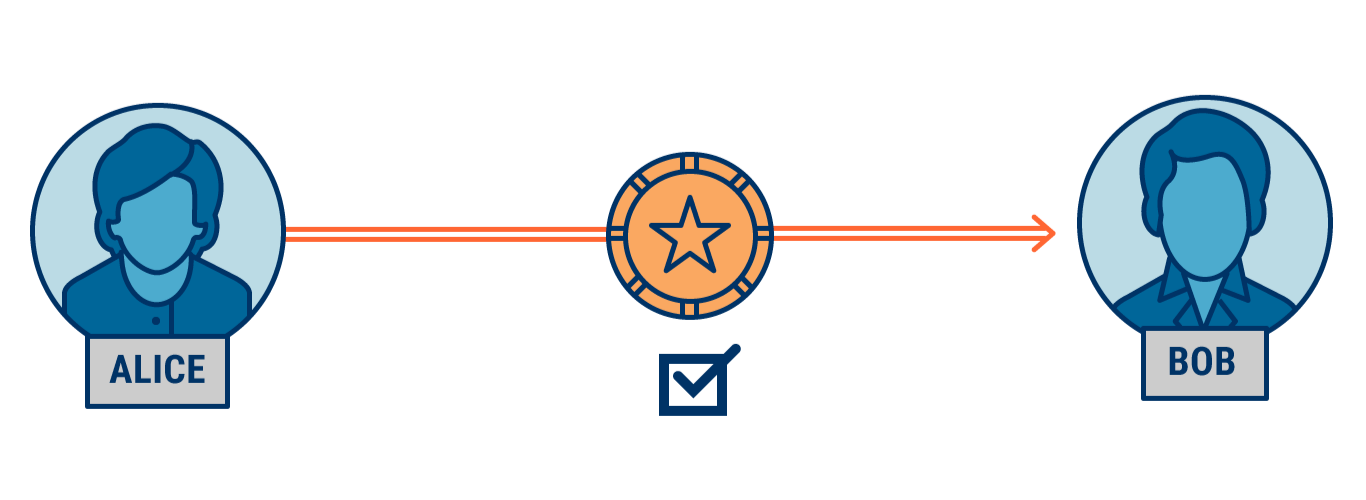
\includegraphics[width=\textwidth]{Figures/blockchain1.png}
        \caption{A physical transaction}
        \label{fig:bc1}
    \end{subfigure}
    ~
    \begin{subfigure}[b]{0.5\textwidth}
        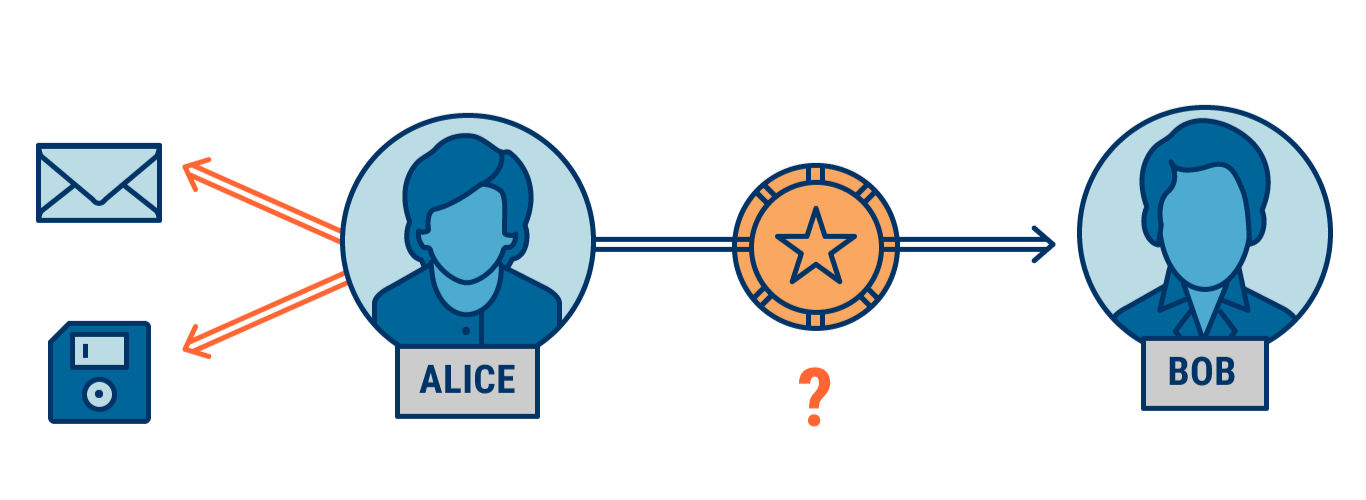
\includegraphics[width=\textwidth]{Figures/blockchain2.png}
        \caption{A digital transaction}
        \label{fig:bc2}
    \end{subfigure}
    ~
    \begin{subfigure}[b]{0.5\textwidth}
        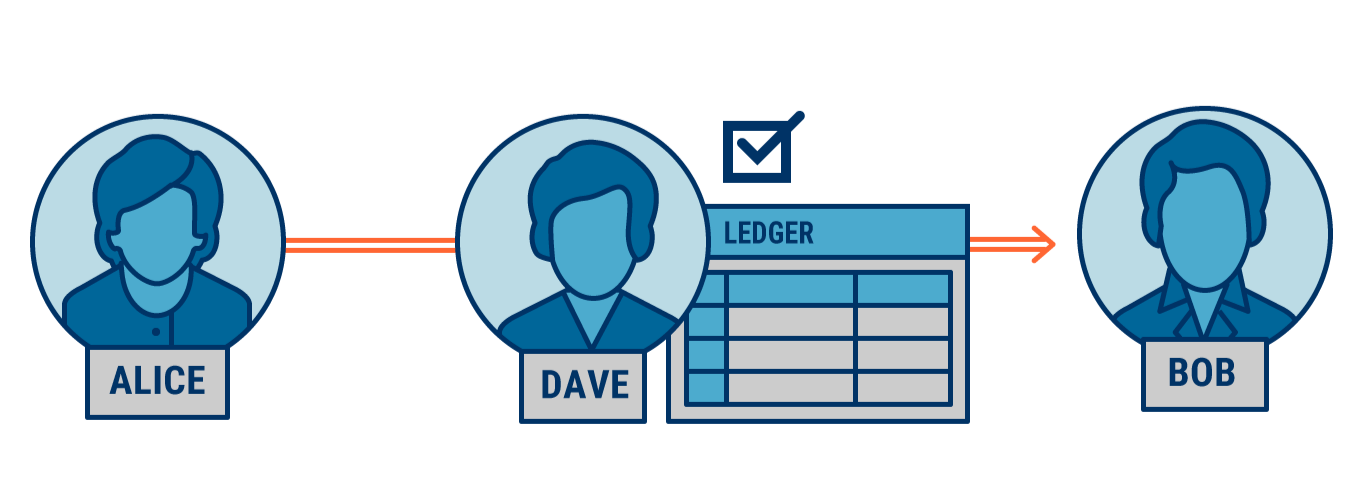
\includegraphics[width=\textwidth]{Figures/blockchain3.png}
        \caption{A digital transaction with ledger}
        \label{fig:bc3}
    \end{subfigure}
    ~
    \begin{subfigure}[b]{0.7\textwidth}
        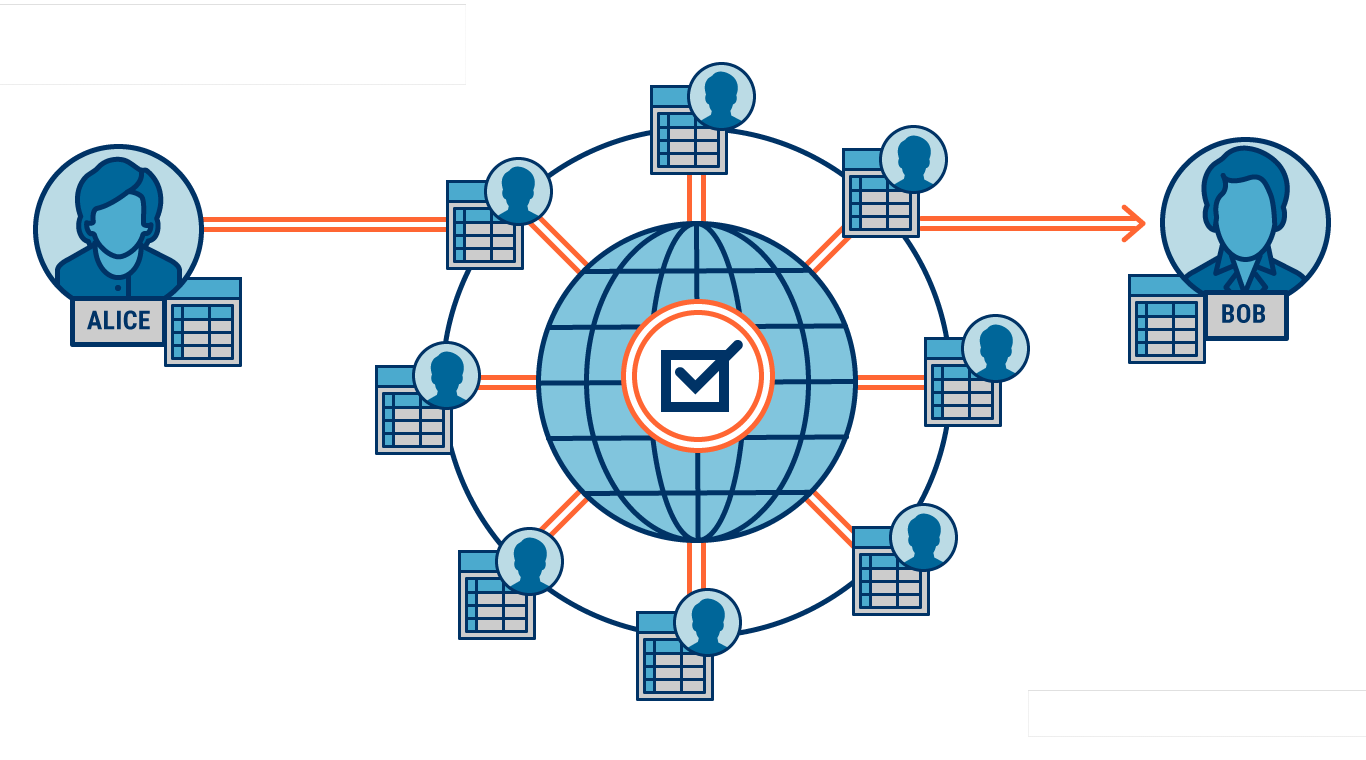
\includegraphics[width=\textwidth]{Figures/blockchain4.png}
        \caption{A decentralized ledger}
        \label{fig:bc4}
    \end{subfigure}
    \caption{Understanding decentralized ledger}
    \label{fig:bc}
\end{figure}

In reference to Figure\footnote{Credits: \url{https://www.cbinsights.com/research/what-is-blockchain-technology/}}
\ref{fig:bc1}, in a physical transaction, the Alice hands Bob a physical arcade coin. Bob now has one coin, and Alice has zero. The transaction is complete. 
If the same transaction is to be performed digitally (Figure \ref{fig:bc2}), Alice would send a string of some bits (corresponding to the desired amount) to Bob. 
Now, since it is just a string of bits, what is the guarantee that Alice would not reproduce that same string of bits in her mail or hard-disk?
If this happens, it would mean that although Alice sent Bob the amount, Alice still possesses the same amount. 
This clearly is a violation.
To tackle this, we must have a ledger or a record of all transactions between Alice and Bob. 
When Alice gives Bob the digital token, the ledger records the transaction (Figure \ref{fig:bc3}). 
Bob has the token, and Alice does not. Let us call the one who maintains this ledger as Dave.
This setup assumes that Dave is a trusted middleman for maintaining ledger. 
Now, what if Alice bribes Dave to erase her transaction? What if Dave decides to charge a fee that neither Alice or Bob want to pay? 
What happens when Alice and Bob cannot trust the third party? This results in a decentralized and public ledger system (Figure \ref{fig:bc4}). 
When a lot of people have a copy of the same ledger, it becomes very difficult to tamper the system and cheat. 
This works because everyone is holding a copy of the same digital ledger and more the number of trusted people holding this ledger, the stronger it becomes.


Blockchain technology offers a way for untrusted parties to reach a consensus on a common digital history. The World Bank defines Blockchain as follows \cite{natar17}:

\begin{definition}[Blockchain]
    A `blockchain' is a particular type of data structure used in some distributed ledgers
    which stores and transmits data in packages called ``blocks'' that are connected to each
    other in a digital `chain'. 
\end{definition}

Blockchains employ cryptographic algorithms to record and synchronize data across a network in an unchangeable manner. The \textit{state} of the Blockchain is the current status of the ledger visible to public. 
In case of Bitcoin, any independent observer can verify the state of the blockchain as well as the validity of all the transactions on the ledger.
This is a \textit{serious} limitation for Bitcoin and could possibly prohibit many use cases.
As an example, if employees of a company were to receive their salaries in bitcoin, would they agree if their salaries were published on the public blockchain? 
This naturally demands for a transaction system which preserves \textit{anonymity} and \textit{confidentiality}.


\section{Notion of Privacy on a Blockchain}

The very concept of having all the information about transactions (predominantly financial) public via a distributed ledger or a blockchain demands for privacy and anonymity of the users.
Before we talk about privacy on the blockchain, it is necessary to understand what we do mean by terms like \textit{privacy} and \textit{anonymity}.
Modern day cryptography is based on the following primary functions \cite{kesler98}:
\begin{enumerate}
    \item[(i)] \textit{Privacy/confidentiality}: To ensure that no one can read or access the message except the intended receiver
    \item[(ii)] \textit{Authentication}: Proving one's identity
    \item[(iii)] \textit{Integrity}: Ensuring that the message intended to be received by the receiver is not altered in the path
    \item[(iv)] \textit{Non-repudiation}: A protocol for checking if a message was actually generated by the sender
    \item[(v)] \textit{Key exchange}: The protocol which determines how key(s) are shared between the sender and the receiver
\end{enumerate}

All of the above functions form an necessary part of a cryptographic system. A well-designed system ensures all of the above functions are taken care of considering the computational bounds for carrying out any protocol.
In a confidential transaction, it is desirable to have \textit{confidentiality} and \textit{anonymity}. 
This means that in a valid confidential transaction, the identity of the sender and receiver must be confidential and the amounts transferred must also be hidden. 
The idea of having such private transactions in digital currencies could be traced back to David Chaum's work on blind signatures \cite{chaum82}.
A similar concept of privacy is required in the blockchain framework. 
The digital assets owned by users must not be publicly visible.
There should be a mechanism to unlink the identity of a user with his or her digital identity, i.e. public key address. 
The interaction between the sender and the receiver in a transaction must not reveal anything to them other than the amounts being transferred.
A user must not be able to reuse his or her digital assets. 
Making the transactions digital and public at the same time brings about several challenges in ensuring that the above requirements are being satisfied.
Active research is still being pursued in the direction of not only solving such practical problems but to do them efficiently and in a scalable manner.

\section{Cryptocurrency Exchanges}

The rise of cryptocurrencies began with the inception of Bitcoin in 2009. Since
then, several cryptocurrencies with better privacy and security guarantees are being
developed. Cryptocurrencies gained popularity among general masses with the establishment of cryptocurrency exchanges.
Also known as digital currency exchanges or crypto exchanges, they are essentially businesses that allow customers to trade
cryptocurrencies or digital currencies for other assets including conventional fiat
money or different digital currencies. 
From a customer point of view, exchanges not only made owning cryptocurrencies possible to non-miners but also provided them with fast trading platforms for transactions within cryptocurrencies and fiat.
Customers were also provided with custodial wallets freeing them from the hassle of storing and remembering private keys.
In the early days of cryptocurrency, crypto exchanges were very few and less-known, but not too long ago their number increased dramatically and they became an integral part of the cryptoeconomic ecosystem. 
They were responsible for the boost in the transaction volumes of the vast majority of the cryptocurrency sales and liquidity.

\subsection{Hacks and Frauds of Exchanges}

The downside of cryptocurrency exchanges is that they are required to
store sensitive information of customers like the private keys and account balances.
If in case an exchange is hacked, it might result in loss of customer-owned cryptocurrency assets.
There have been many high-profile hacks over the years, many of which went unnoticed for some time \cite{Cryptohacks}.
In 2014, one of the biggest Bitcoin exchanges Mt.Gox lost almost 750,000 of its customers' bitcoins and around 100,000 of its own bitcoins, totaling around 7\% of all bitcoins back then, and worth around \$473 million, leading to filing of bankruptcy.
There have been cases where exchanges lure customers into buying digital assets in return for fiat currency, but do not allocate any digital assets in reality.
Such exit scams by exchanges have led to huge losses of customer and investor funds \cite{Robert2020}.

Although having a fool-proof method to avoid such hacks might be a difficult task, proof of solvency is one way to uphold the trust of customers.
A proof of solvency is the guarantee by the exchange that it owns reserves at least as much as its total liabilities towards customers. 
In this way, even after cases of hacking, the exchange could repay its liabilities to the customers.


\section{Proof of Solvency}

An exchange is said to be solvent if it owns assets at least as much as its liabilities.
An exchange proving solvency convinces its customers that in an unfortunate case of a hack or a fraud, it could reimburse the lost customer funds through its own assets.
A proof of solvency consists of two parts: proof of reserves and proof of liabilities.
The former proves the assets owned by the exchange while the latter shows the total liabilities of the exchange towards its customers.

The challenge in designing proof of solvency is to maintain privacy of the exchange as well as the customers.
Proof of reserves protocols in \cite{Dagher2015,Dutta2019a,Dutta2019b} publish a Pedersen commitment to the total assets owned by the exchange.
Pedersen commitments are a cryptographic way of hiding secret messages or amounts. We will describe Pedersen commitments in detail in the next chapter.
Suppose an exchange publishes $C_{\text{res}}$ as a Pedersen commitment to its total reserves $a_{\text{res}}$.
Similarly, it could publish a Pedersen commitment to its total liabilities $a_{\text{liab}}$ as $C_{\text{liab}}$ using customer data as described in \cite{Dagher2015}.
However, this proof of reserves in \cite{Dagher2015} requires each customer to individually verify that his or her amount is included in the proof of liabilities.
If a customer fails to verify his or her amount, the exchange in principle could hide the particular customer's data to shrink its liabilities.
Chalkias \textit{et al}. \cite{Chalkias2020} recently proposed a scheme called Distributed Auditing Proofs of Liabilities (DAPOL) which addresses this concern. 
% DAPOL uses deterministic sparse Merkle tree combined with range proofs on the commitment to each customer's amount and a Pedersen commitment to $a_{\text{liab}}$. 
DAPOL uses private information retrieval to ensure the inclusion proof by every customer.
Therefore, given the Pedersen commitments to reserves and liabilities of an exchange, it can prove solvency by proving that the quantity $C_{\text{res}} \cdot C_{\text{liab}}^{-1}$ commits to a non-negative amount and thus, $a_{\text{res}} - a_{\text{liab}} \ge 0$.
This suffices because $C_{\text{res}} \cdot C_{\text{liab}}^{-1}$ is a Pedersen commitment to $a_{\text{res}} - a_{\text{liab}}$ due to the homomorphic property of Pedersen commitments.

\subsection{Proof of Reserves}

A proof of reserves protocol is used by a cryptocurrency exchange to prove that it owns a certain amount of cryptocurrency. 
If privacy of the amount or outputs owned by the exchange is not an issue, then proving reserves involves a straightforward proof of the ability to spend the exchange-owned outputs (for example, see \cite{BlockstreamProofOfReserves}). 
The simplest way to publish a proof of reserves for an exchange is to reveal all the addresses or account details it owns so that the customers are convinced about the assets owned by the exchange.
Another way could be to send all the reserves it owns from all its addresses to a single addresses it owns.
If amounts involved in a transaction are public as in the case of Bitcoin, such a self-transaction would be a proof of the exchange's reserves.
For example, in 2011, Mt.~Gox cryptocurrency exchange transferred 424,242 bitcoins from its wallets to a previously revealed Bitcoin address \cite{MtGoxWikipedia}.
Information of an exchange's addresses or accounts and the total assets it owns are crucial for aspects of its business.
Thus, non-private proof of reserves protocols are unlikely to be adopted by exchanges as they may reveal business strategy. 
Privacy-preserving proof of reserves protocols have been proposed for Bitcoin \cite{Decker2015,Dagher2015}, Monero \cite{Dutta2019a}, and MimbleWimble \cite{Dutta2019b}. 
In fact, the protocols proposed by Decker \textit{et al} \cite{Decker2015} and Dagher \textit{et al} \cite{Dagher2015} go one step further and give a privacy-preserving proof of solvency, i.e.~they prove that the reserves owned by the exchange exceed its liabilities towards its customers. 
However, the work in \cite{Decker2015} relies on a trusted hardware assumption. And the proof of liabilities protocol in \cite{Dagher2015} is secure only if every exchange customer checks the proof. 
In general, it seems that designing proof of reserves protocols is easier than designing proof of liabilities protocols as the former depend only the blockchain state while the latter depend on the exchange's private customer data.
% An exchange can reduce its reported liabilities by censoring its customer list.

Even without a robust proof of liabilities protocol, a privacy-preserving proof of reserves protocol based on homomorphic commitments is valuable. 
% For example, the proof of reserves protocols in \cite{Dagher2015,Dutta2019a,Dutta2019b} generate a Pedersen commitment $C_{\text{res}}$ to the amount of reserves. 
Exchanges can easily prove that $C_{\text{res}}$ is a commitment to an amount which exceeds a base amount $a_{\text{base}}$. While the base amount may not be exactly equal to the total liabilities of the exchange, it can be based on the trade volume data published by the exchange \cite{Coinmarketcap}. 
This technique will help early detection of exchange hacks and exit scams. 
For example, in Februrary 2019 the Canadian exchange QuadrigaCX claimed that it had lost access to wallets containing customer funds due to the death (in December 2018) of their CEO who had sole custody of the corresponding passwords and keys. But an official investigation found that the wallets had been empty since April 2018, several months before the CEO's death \cite{QuadrigaCXEmpty, EYThirdReport}. This discrepancy would have been detected earlier if the exchange had been required to give perioidic proofs of reserves.
Realising the importance of proof of reserves as a tool in raising customer confidence in crypto-exchanges leads us to the need for building better proofs in terms of privacy, scalability and performance.    

The main challenge in design of proofs of reserves is to preserve privacy and confidentiality of exchanges but at the same time convince customers about an exchange's actual asset ownership.
Regaining \textit{trust} of the customers without compromising exchanges' \textit{privacy} is the primary motivation behind the design of better proofs of reserves. 
Advanced cryptographic techniques make it possible to design proofs of reserves which reveal \textit{nothing} beyond an assertation of the form:
\begin{center}
    \textit{Exchange X owns ? amount of the cryptocurrency Y at time t.}
\end{center}
Note that here we do not intend to reveal even the total amount. 
A publicly verifiable proof backing up such a claim is a cryptographic tool known as a \textit{Non-Interactive Zero-Knowledge} proof.

\section{Organization of the Thesis}

After motivating the problem we are trying to address in this work, we will briefly describe the cryptographic primitives necessary to understand our work in Chapter \ref{chap:crypto_prelims}.
We briefly discuss the literature in Chapter \ref{chap:lit} which is necessary to understand the latter chapters.  
In Chapter \ref{chap:revBP}, we start with outlining the details of Grin and existing state-of-the-art proof of reserves protocol for MimbleWimble-based cryptocurrencies. 
We describe \RB - a novel proof of reserves protocol for MimbleWimble-based cryptocurrencies in Chapter \ref{chap:revBP} along with its security properties.
We present the Grin outputs' amount confidentiality analysis in Chapter \ref{chap:grin-ub}.
Finally, we discuss all the security proofs in detail in the Appendix \ref{scn:appendix}.  


%%


%%% Local Variables: 
%%% mode: latex
%%% TeX-master: "../mainrep"
%%% End: 
